\documentclass[a4paper]{article}

\usepackage{tikz}
\usetikzlibrary{arrows, calc, positioning}

\begin{document}
\begin{center}
	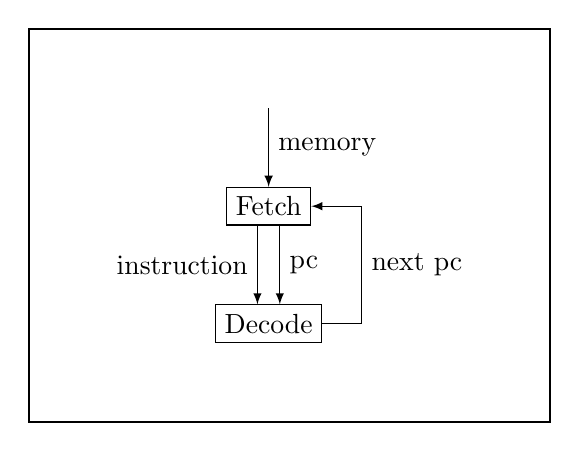
\begin{tikzpicture}[>=latex]
		\node[draw] (fetch) {Fetch};
		\node[draw] [below=of fetch] (decode) {Decode};

		\draw[->] (fetch.north) ++(0,1) -- node[right] {memory} (fetch.north);
		\draw[->] (fetch.240)   -- node[left]  {instruction} (fetch.240|-decode.north);
		\draw[->] (fetch.300)   -- node[right] {pc}          (fetch.300|-decode.north);
		\draw[->] (decode.east) -- ++(.5,0) |- node[right, pos=0.25] {next pc} (fetch.east);

		\draw[thick] (current bounding box.south west) ++(-1,-1) rectangle ($(current bounding box.north east)+(1,1)$);
	\end{tikzpicture}
\end{center}
\end{document}